\setcounter{page}{1}
\section*{Zielsetzung}
Im Versuch 353 sollen Relaxationsphänomene untersucht werden. Hierbei handelt es sich um Effekte, die bei der Rückkehr eines
Systems in seinen Gleichgewichtszustand auftreten. Derartige Erscheinungen lassen sich beispielsweise in der Mechanik, Thermodynamik
und Elektronik beobachten. Im Versuch soll konkret das Relaxationsverhalten eines RC-Kreises beobachtet und diskutiert werden.
\section{Theorie}
\subsection{Entladekurve eines Kondensators}
Die Spannung $U\ua{C}$ an einem Kondensator stellt sich als Quotient zwischen der auf ihm gespeicherten Ladung $Q$ und seiner Kapazität $C$ dar:
\begin{equation}
  U\ua{C} = \frac{Q}{C} \quad \Leftrightarrow \quad Q = C\, U\ua{C}.
  \label{eq: ladung}
\end{equation}
Für den durch diese Potentialdifferenz hervorgerufenen Strom $I$ durch einen in Reihe geschalteten Widerstand $R$ gilt nach dem ohmschen Gesetz
\begin{equation}
  I = -\frac{U\ua{C}}{R}.
  \label{eq: strom}
\end{equation}
Der Strom ist also so gerichtet, dass er letztendlich zum Ladungsausgleich führt. Mittels Differentiation der Gleichung \eqref{eq: ladung} und anschließendem
Gleichsetzen mit \eqref{eq: strom} erhält
man eine gewöhnliche Differentialgleichung für den zeitlichen Verlauf der Spannung $U\ua{C}(t)$:
\begin{equation}
  \frac{\dif{U\ua{C}}}{\dif{t}} + \frac{1}{RC}U\ua{C} = 0,
\end{equation}
die durch eine exponentielle Funktion gelöst wird.
\begin{equation}
  \label{eq:entlade_kurve}
  U\ua{C} = A \exp\left(-\frac{t}{RC}\right)
\end{equation}
Der Wert $RC$ wird wird als charakteristische Zeitkonstante des Relaxationsprozesses bezeichnet. Innerhalb dieser Zeitspanne ändert
sich die Spannung um den Faktor
\begin{equation}
  \frac{U\ua{C}(t = RC)}{A} = \frac{1}{e}.
\end{equation}
\subsection{Relaxationsprozesse unter Einfluss periodischer Auslenkungen}
Wird gemäß Abbildung \ref{fig: aufbau_2} eine sinusförmige Wechselspannungsquelle $U(t) = U_0sin(\omega t)$ in den RC-Kreis integriert, kommt es zu frequenzabhängigen
Effekten. Zwischen Generator- und Kondensatorspannung tritt eine Phasenverschiebung $\varphi(\omega)$ auf, die durch folgende Gleichung
beschrieben wird:
\begin{equation}
  \varphi(\omega) = \arctan(-\omega RC).
  \label{eq: phase_theorie}
\end{equation}
\FloatBarrier
\begin{figure}
  \centering
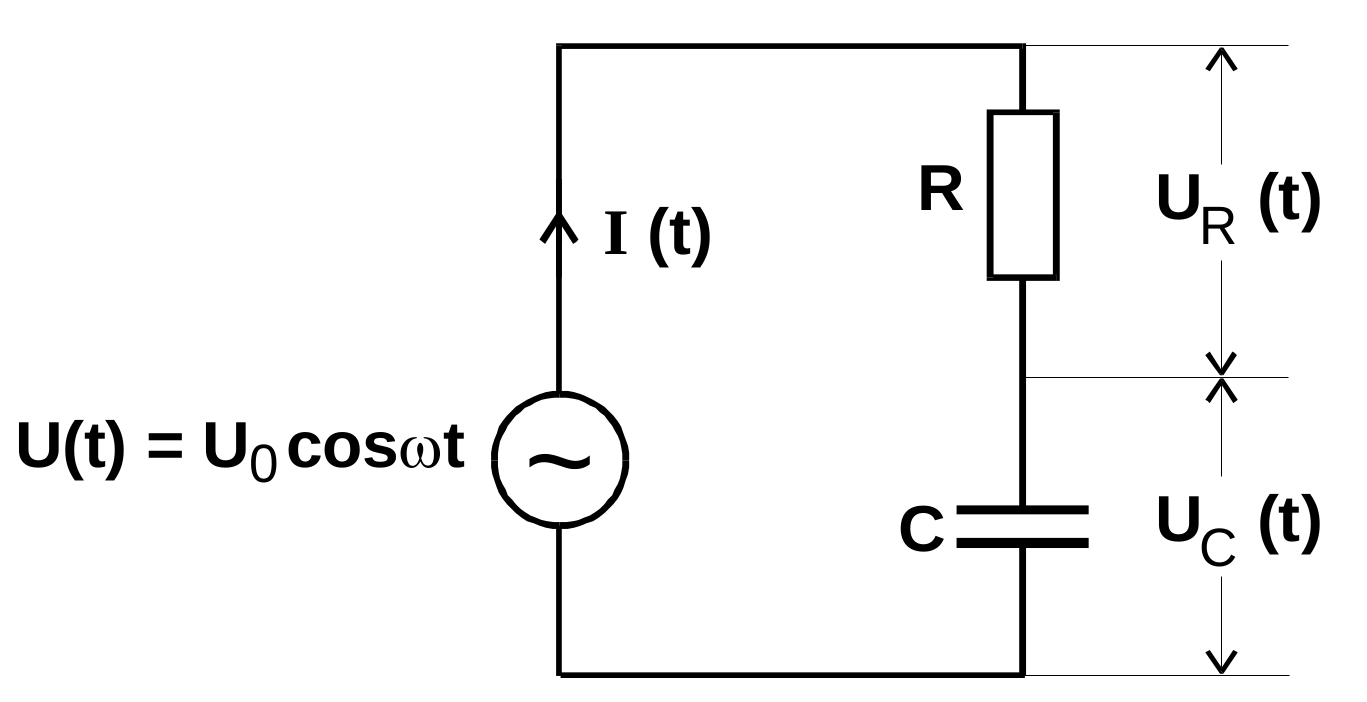
\includegraphics[width = 0.5\textwidth]{pics/aufbau_2.png}
\caption{Aufbau zur Diskussion des Einflusses einer Wechselgeneratorspannung in einem RC-Kreis\cite{anleitung353}. }
\label{fig: aufbau_2}
\end{figure}
Des Weiteren ist ebenfalls die Amplitude $A(\omega)$ der Kondensatorspannung von der Frequenz abhängig. Hierfür ergibt sich der Zusammenhang:
\begin{equation}
  A(\omega) = \frac{U_0}{\sqrt{1 +\omega^2R^2C^2}}.
  \label{eq: amplitude_theorie}
\end{equation}
Man erkennt also, dass für kleine Frequenzen sowohl Phasen- als auch Amplitudendifferenz zwischen Erregender und Angeregter Spannung verschwinden.
Für große Frequenzen hingegen nähert sich die Amplitude null an und die Phasendifferenz geht gegen $\frac{\pi}{2}$. Diese Gegebenheiten sollen
im Versuch überprüft werden. Um die Ergebnisse später in einer Polarebene einzeichnen zu können, werden die Formeln \eqref{eq: phase_theorie} und
\eqref{eq: amplitude_theorie} benutzt, um die Amplitude $A$ als Funktion von Frequenz und Phase darzustellen:
\begin{equation}
\frac{A(\varphi, \omega)}{U_0} = \cos\left[\varphi(\omega)\right].
  \label{eq: amplitude_phase}
\end{equation}

\subsection{Integratoreigenschaft des RC-Kreises}
Gemäß der Maschenregel gilt für die Spannungen im Stromkreis \ref{fig: aufbau_2}:
\begin{equation}
  U(t) = RC\,\frac{\dif{U\ua{c}(t)}}{\dif{t}} + U\ua{C}(t).
\end{equation}
Ist nun die Frequenz wesentlich höher als der Term $(RC)^{-1}$, so kann gemäß \eqref{eq: amplitude_theorie} der Term $U\ua{C}$ vernachlässigt werden, womit
sich ergibt:
\begin{equation}
  U(t) = RC\,\frac{\dif{U\ua{c}(t)}}{\dif{t}} \quad \Leftrightarrow \quad U\ua{C}(t) = \frac{1}{RC}\int_0^t U(\bar{t})\dif{\bar{t}}.
\end{equation}
Die Aufbau kann also für hohe Frequenzen zur Integration der Spannung $U(t)$ verwendet werden.
